\begin{appendix} %Anhang
\section{Matlab-Berechnungen}
\subsection{Leistungsfaktor}
\lstinputlisting{appendix/code/Leistungsfaktor.m}

\newpage
\section{Vergleich der Resultate von Plecs und Matlab}

\begin{figure}[ht!]
	\centering
	\subfloat[][]{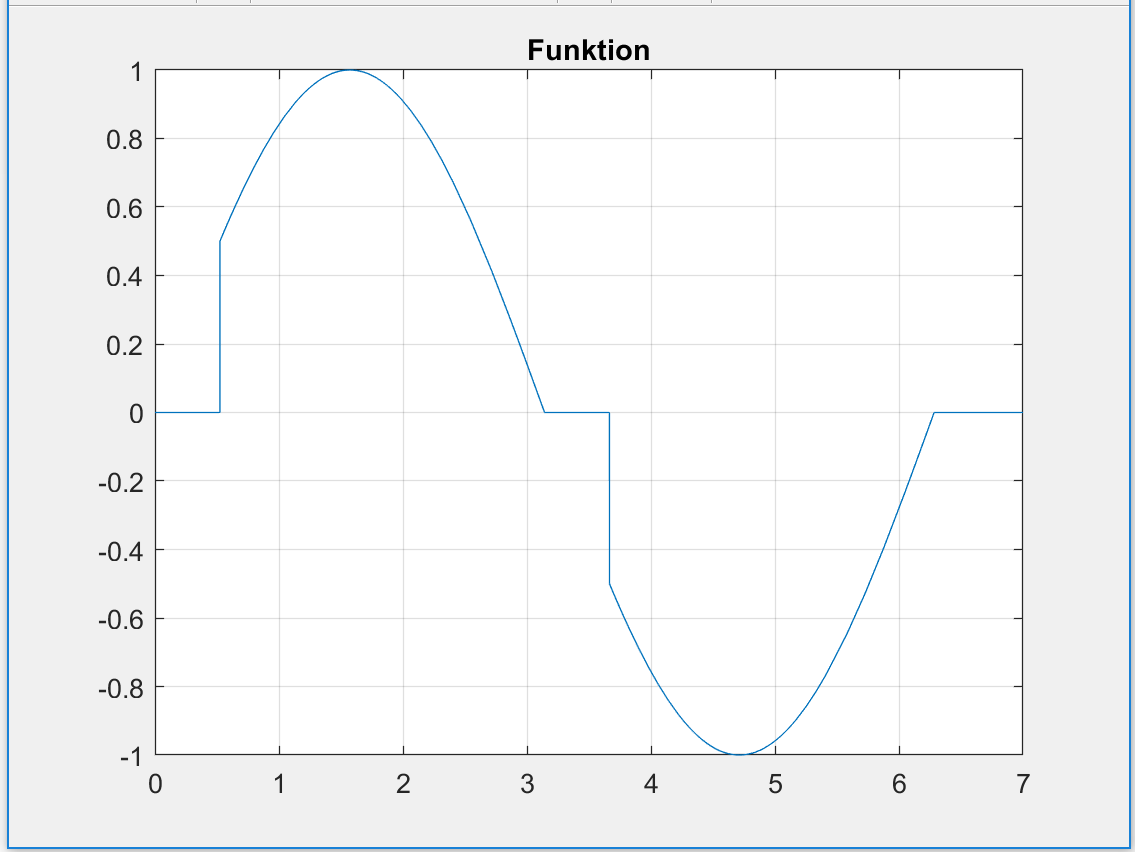
\includegraphics[width=0.4\linewidth]{eingangssignal_30.png}\label{fig:eingangssignal_30}}\qquad
	\subfloat[][]{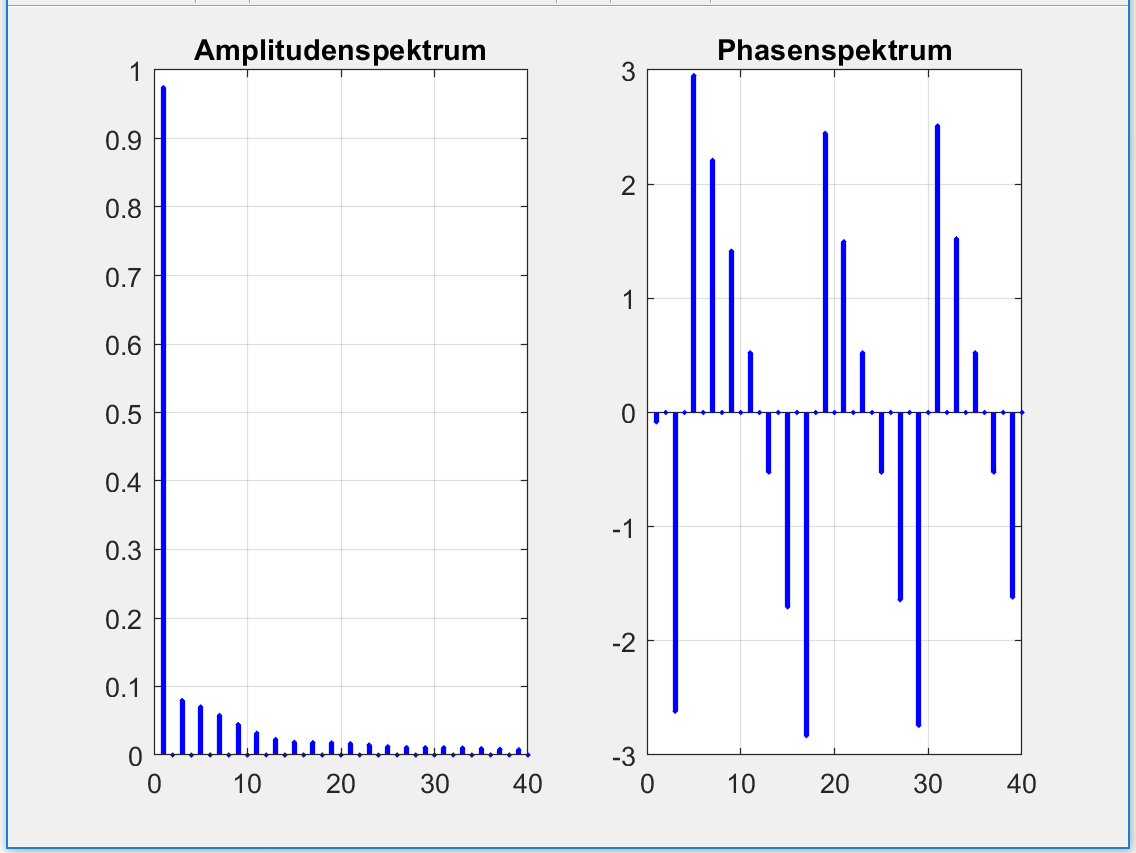
\includegraphics[width=0.4\linewidth]{A_PH_30.png}\label{fig:A_PH_30.}}
	\caption{Phasenanschnittsteuerung mit 30\textdegree (a) Eingangssignal (b) Amplituden- und Phasenspektrum}
	\label{fig:Phasenanschnittsteuerung_mit_30}
\end{figure}

\begin{figure}[ht!]
	\centering
	\subfloat[][]{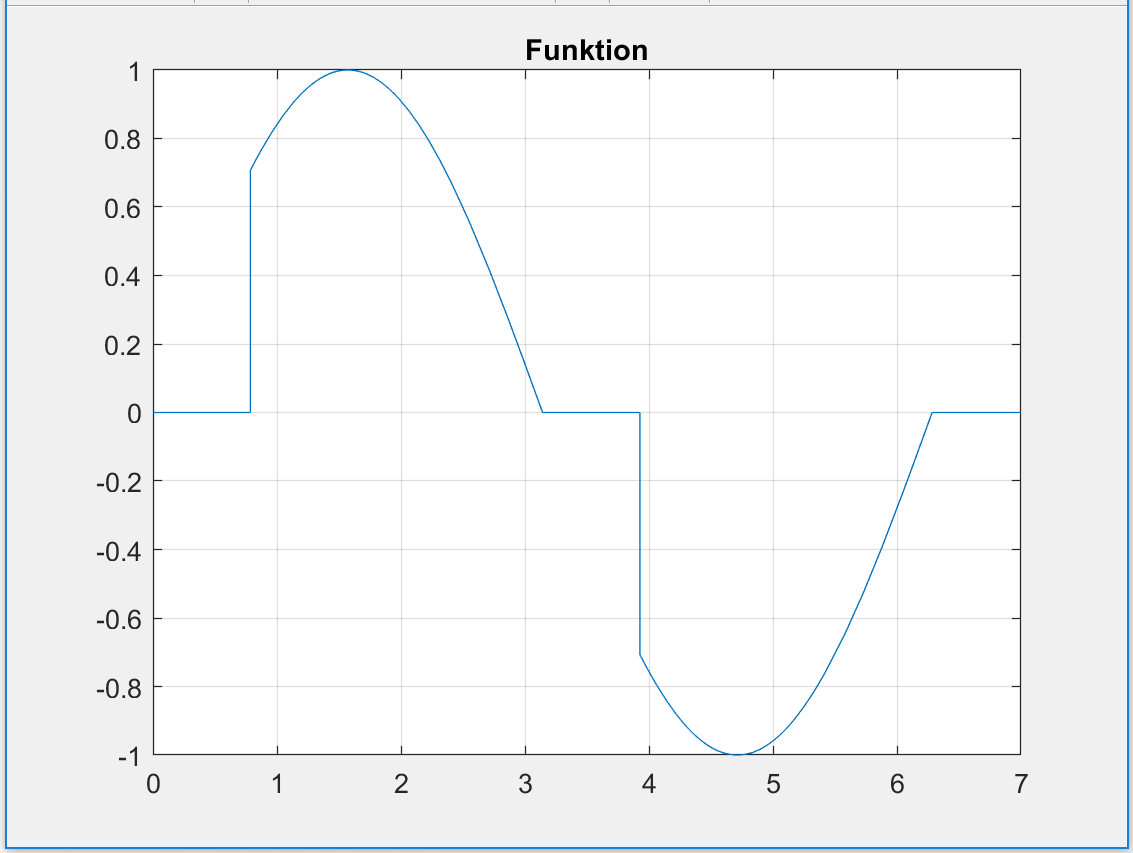
\includegraphics[width=0.4\linewidth]{eingangssignal_45.png}\label{fig:eingangssignal_45}}\qquad
	\subfloat[][]{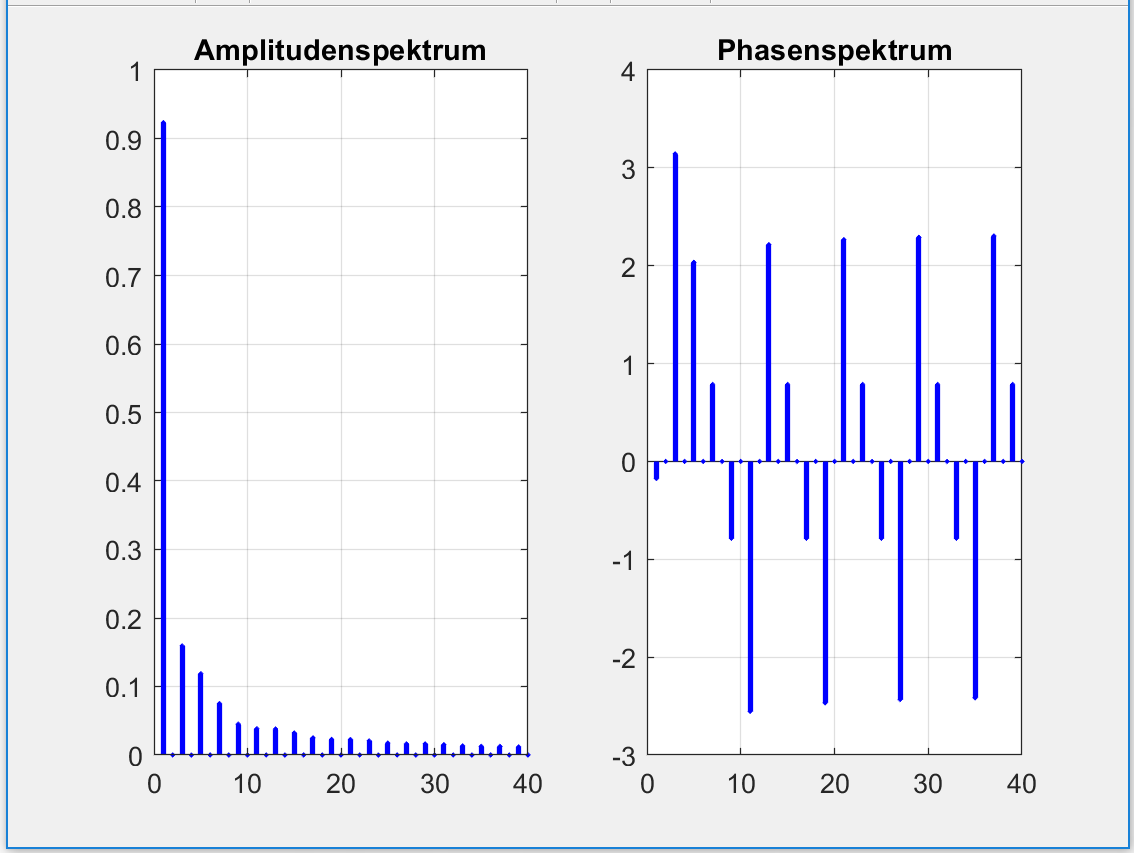
\includegraphics[width=0.4\linewidth]{A_PH_45.png}\label{fig:A_PH_45}}
	\caption{Phasenanschnittsteuerung mit 45\textdegree (a) Eingangssignal (b) Amplituden- und Phasenspektrum}
	\label{fig:Phasenanschnittsteuerung_mit_45}
\end{figure}

\begin{figure}[ht!]
	\centering
	\subfloat[][]{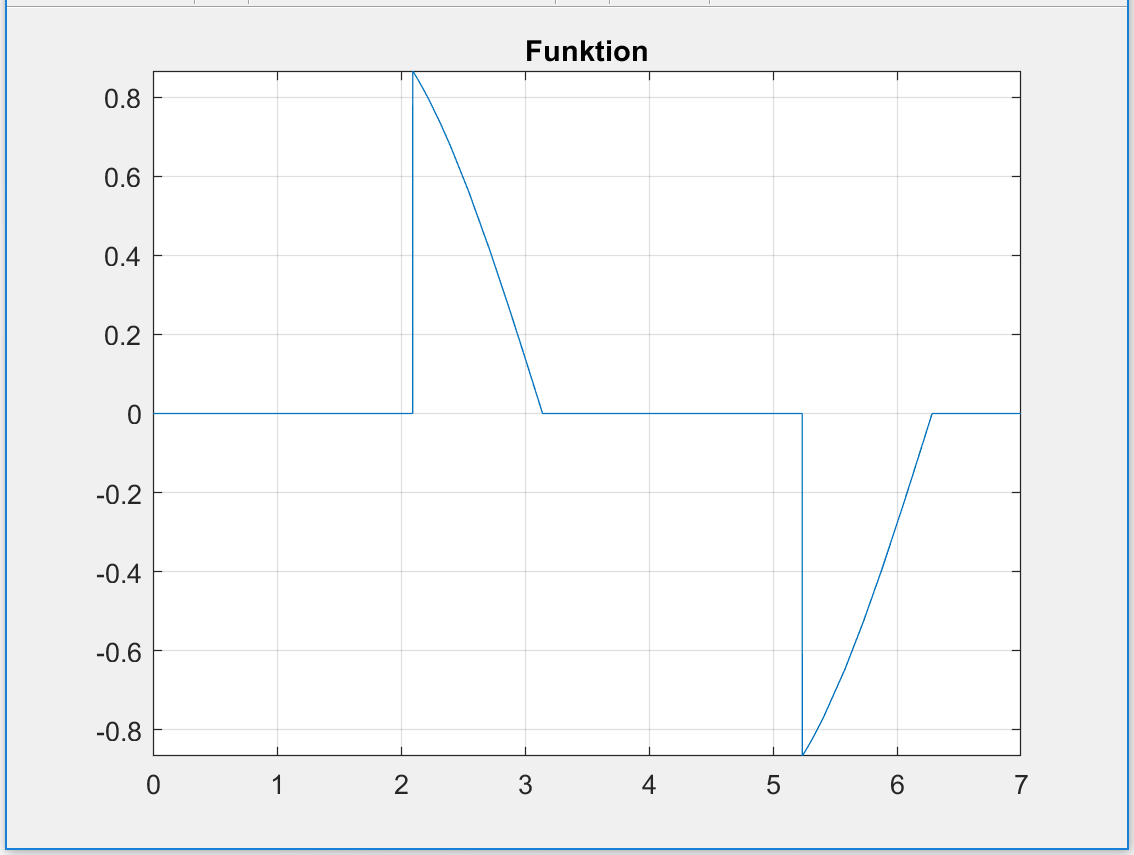
\includegraphics[width=0.4\linewidth]{eingangssignal_120.png}\label{fig:eingangssignal_120}}\qquad
	\subfloat[][]{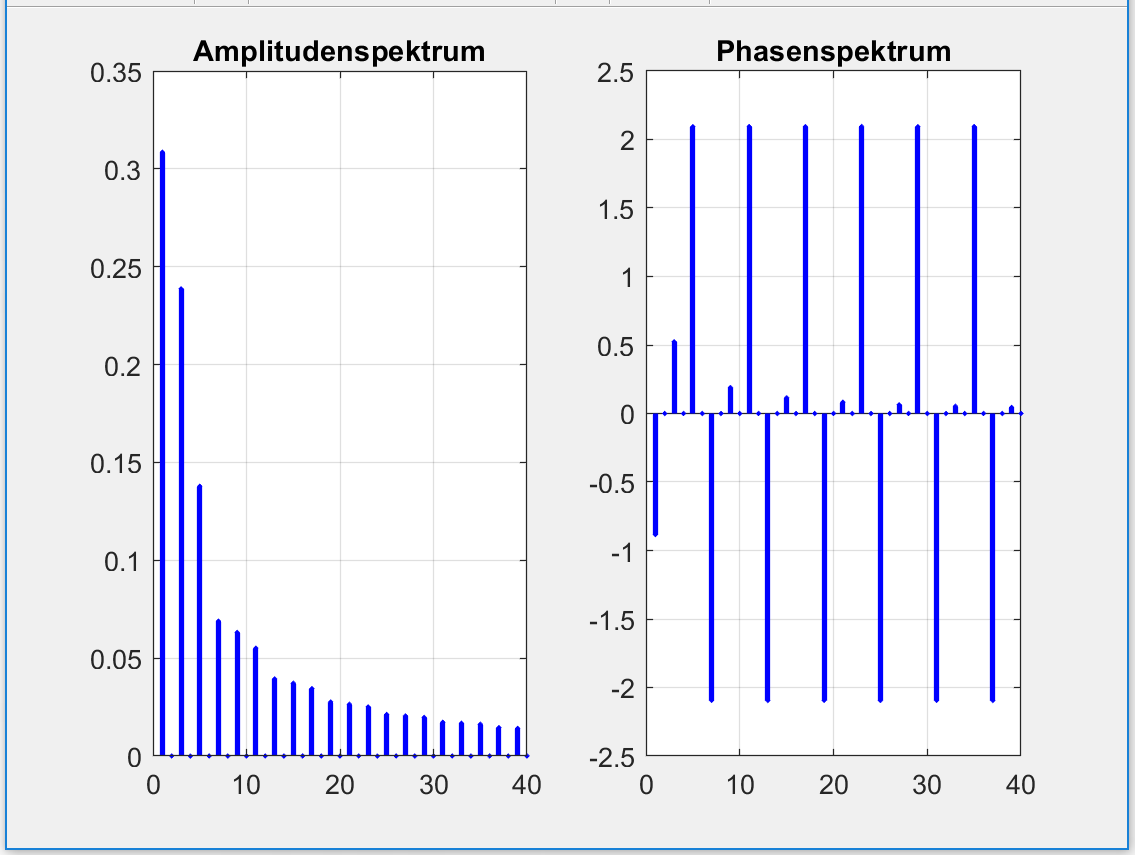
\includegraphics[width=0.4\linewidth]{A_PH_120.png}\label{fig:A_PH_120}}
	\caption{Phasenanschnittsteuerung mit 120\textdegree (a) Eingangssignal (b) Amplituden- und Phasenspektrum}
	\label{fig:Phasenanschnittsteuerung_mit_120}
\end{figure}

\newpage

\begin{figure}[ht!]
	\centering
	\subfloat[][]{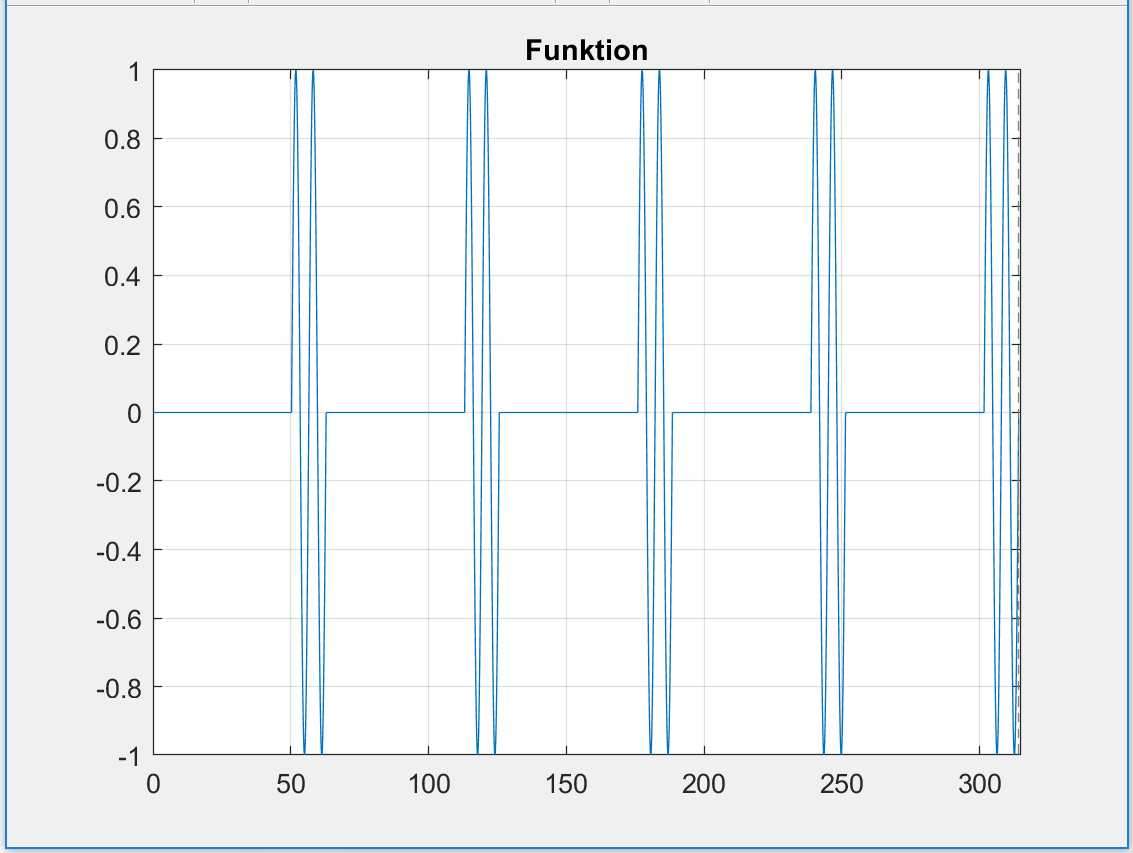
\includegraphics[width=0.4\linewidth]{Schwingungspaket_0_2.png}\label{fig:Schwingungspaket_0_2}}\qquad
	\subfloat[][]{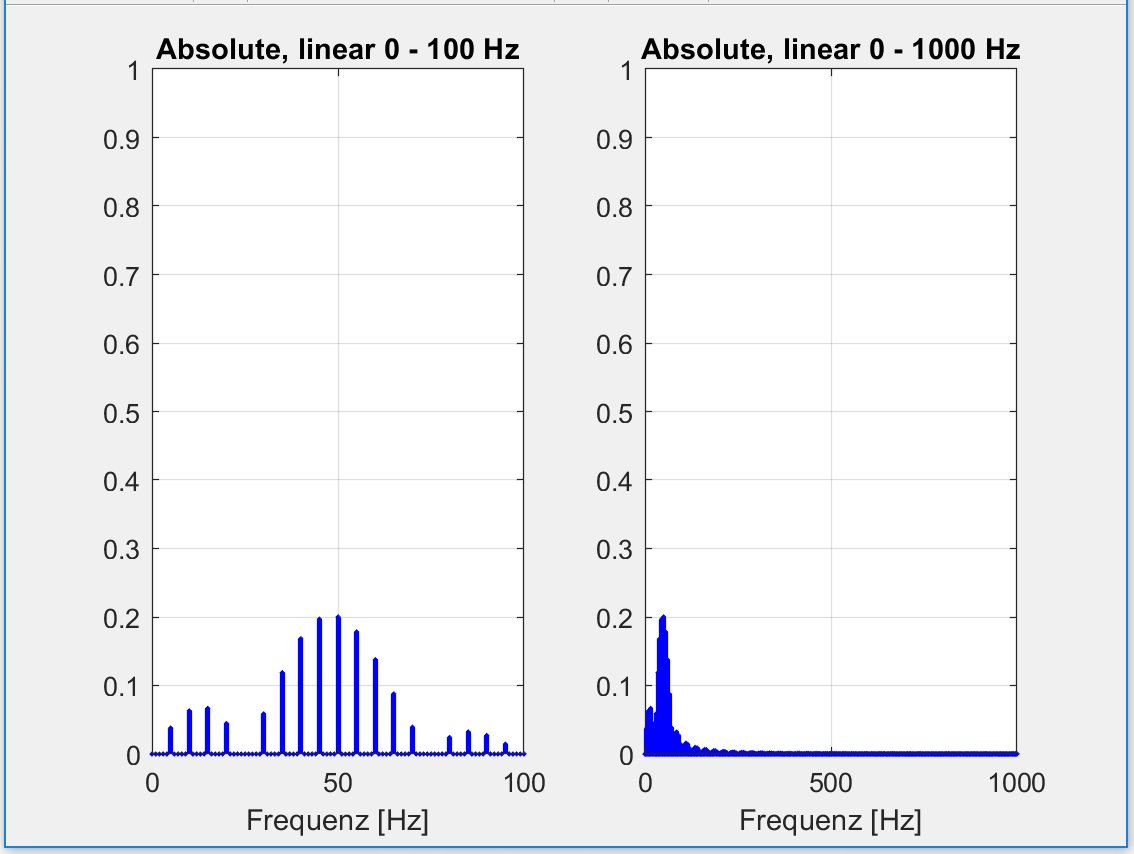
\includegraphics[width=0.4\linewidth]{Oberwellen_0_2.png}\label{fig:Oberwellen_0_2}}
	\caption{Schwingungspaketsteuerung mit duty cycle 0.2 (a) Eingangssignal (b) Amplituden- und Phasenspektrum}
	\label{fig:Schwingungspaketsteuerung_mit_duty_cycle_0_2}
\end{figure}


\begin{figure}[ht!]
	\centering
	\subfloat[][]{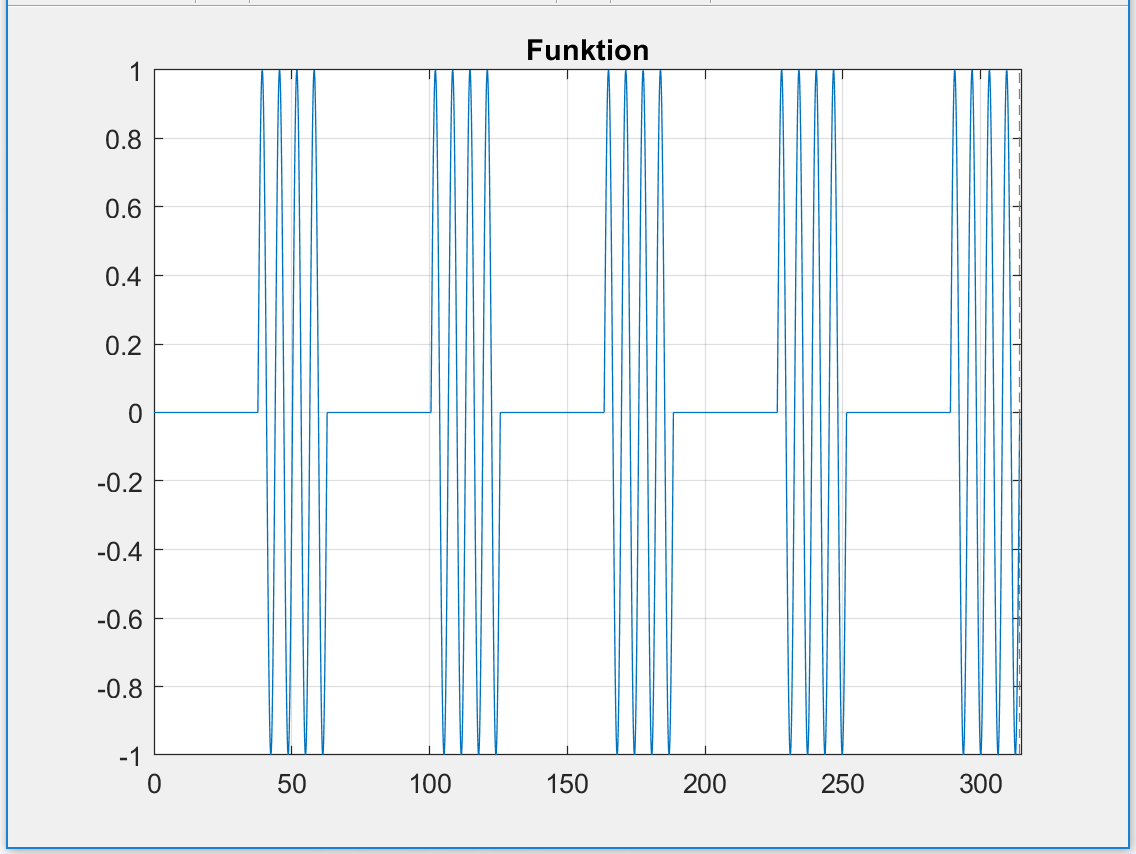
\includegraphics[width=0.4\linewidth]{Schwingungspaket_0_4.png}\label{fig:Schwingungspaket_0_4}}\qquad
	\subfloat[][]{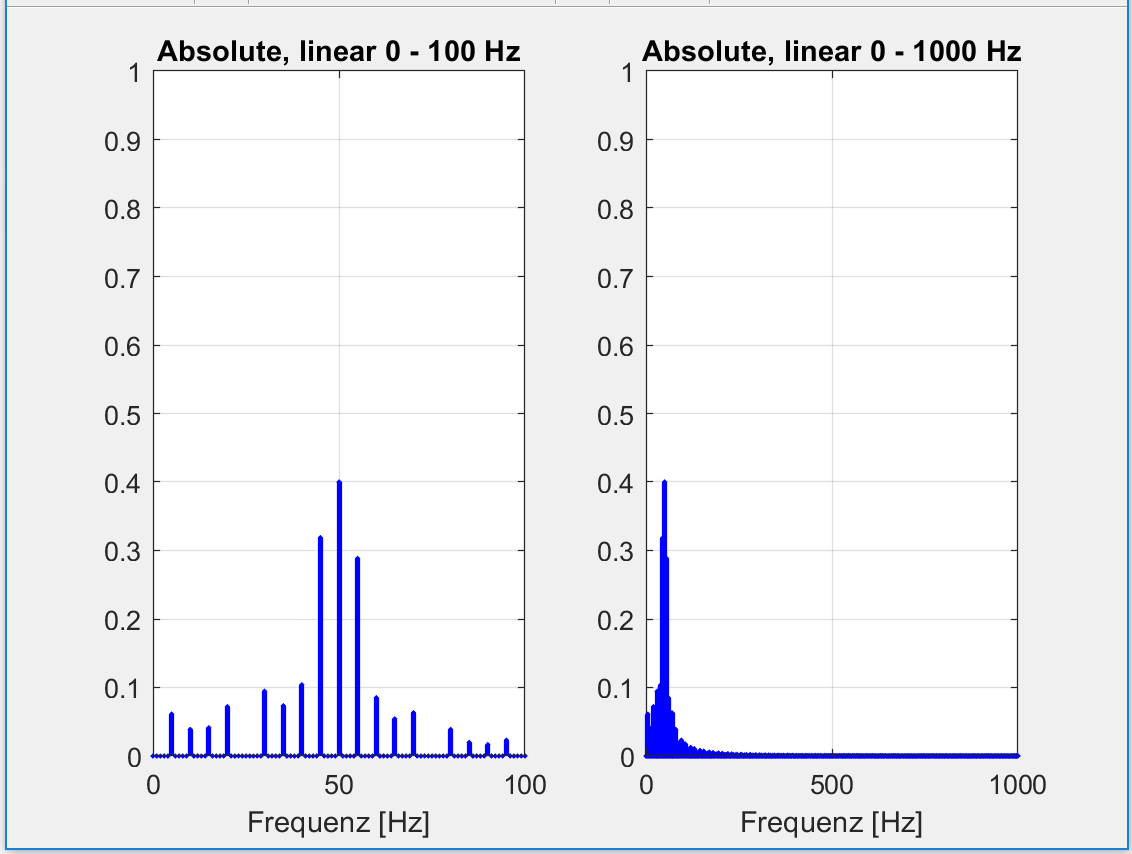
\includegraphics[width=0.4\linewidth]{Oberwellen_0_4.png}\label{fig:Oberwellen_0_4}}
	\caption{Schwingungspaketsteuerung mit duty cycle 0.4 (a) Eingangssignal (b) Amplituden- und Phasenspektrum}
	\label{fig:Schwingungspaketsteuerung_mit_duty_cycle_0_4}
\end{figure}

\begin{figure}[ht!]
	\centering
	\subfloat[][]{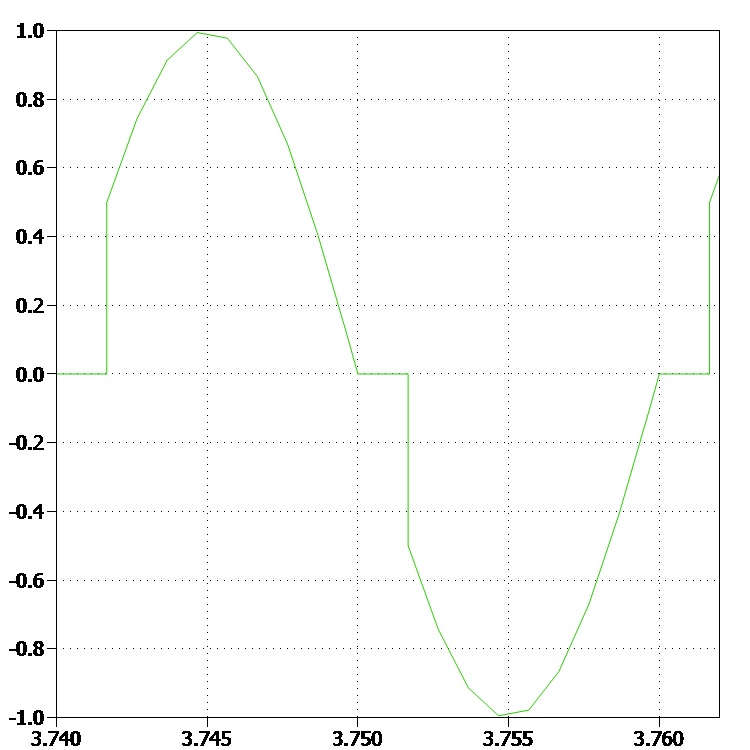
\includegraphics[width=0.32\linewidth]{plecs_phasenanschnitt_pi_6_funktion.png}\label{fig:plecs_phasenanschnitt_pi_6_funktion}}\qquad
	\subfloat[][]{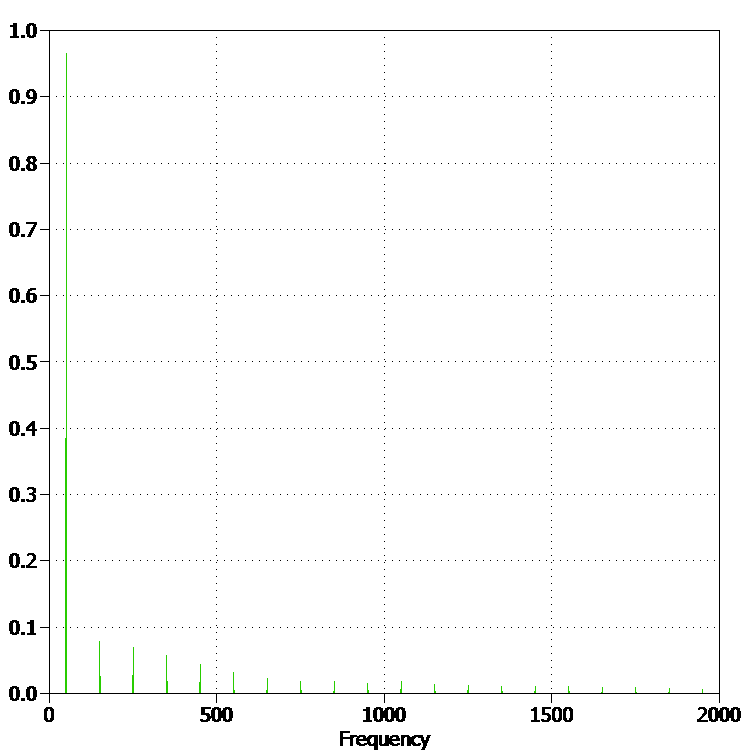
\includegraphics[width=0.32\linewidth]{plecs_phasenanschnitt_pi_6.png}\label{fig:plecs_phasenanschnitt_pi_6}}
	\caption{Phasenanschnitt mit 30\textdegree simuliert mit Plecs (a) Eingangssignal (b) Amplituden- und Phasenspektrum}
	\label{fig:Plecs_mit_phasenanschnitt_30}
\end{figure}

\newpage

\begin{figure}[ht!]
	\centering
	\subfloat[][]{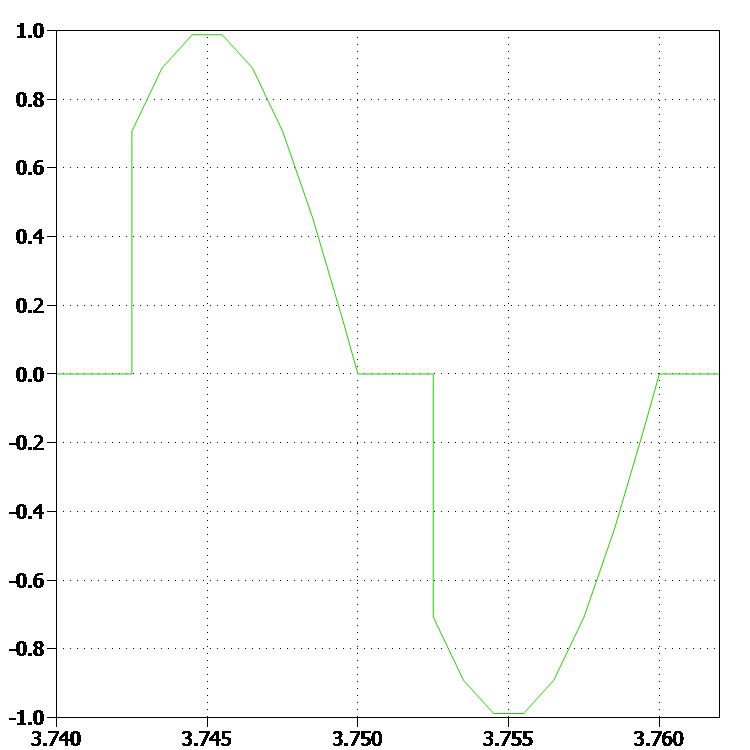
\includegraphics[width=0.32\linewidth]{plecs_phasenanschnitt_pi_4_funktion.png}\label{fig:plecs_phasenanschnitt_pi_4_funktion}}\qquad
	\subfloat[][]{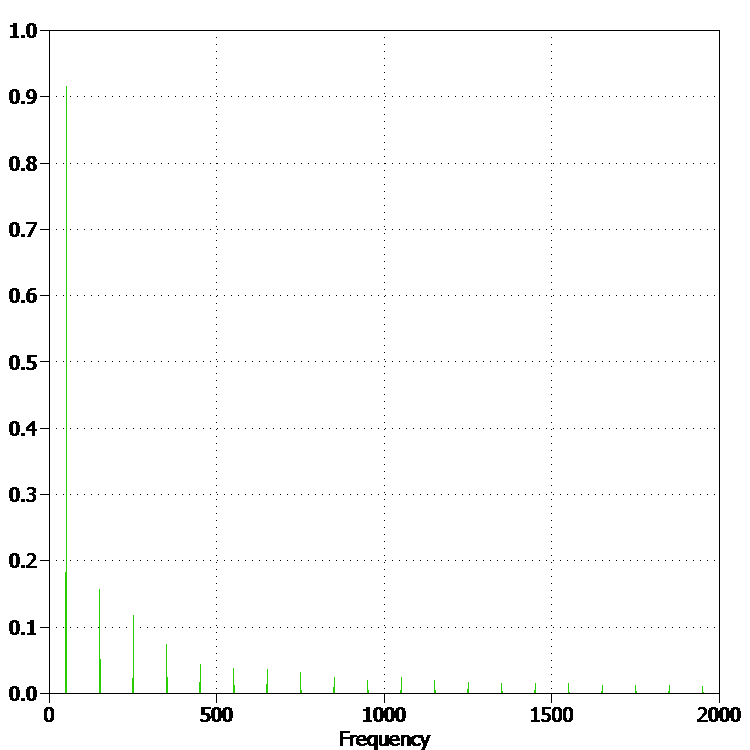
\includegraphics[width=0.32\linewidth]{plecs_phasenanschnitt_pi_4.png}\label{fig:plecs_phasenanschnitt_pi_4}}
	\caption{Phasenanschnitt mit 45\textdegree simuliert mit Plecs (a) Eingangssignal (b) Amplituden- und Phasenspektrum}
	\label{fig:Plecs_mit_phasenanschnitt_45}
\end{figure}


\begin{figure}[ht!]
	\centering
	\subfloat[][]{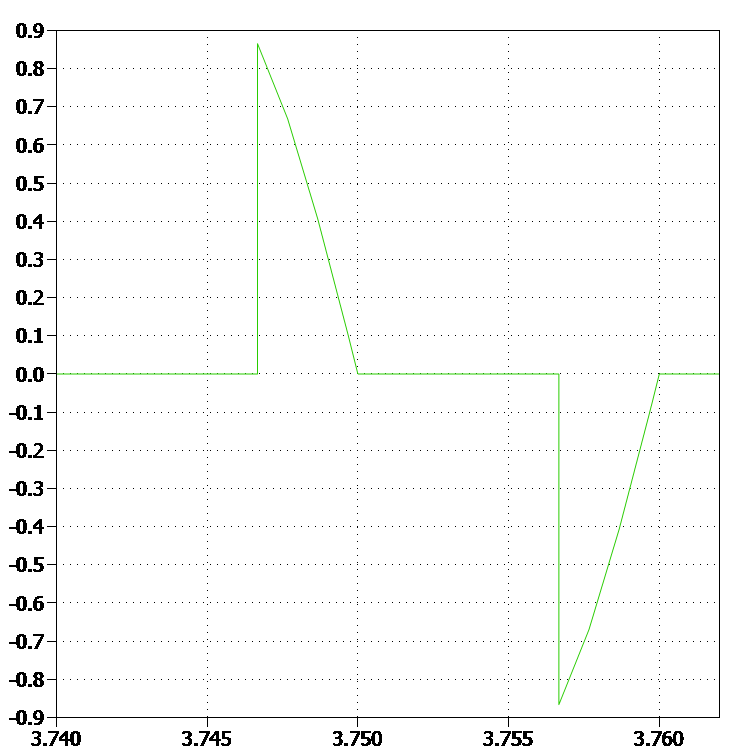
\includegraphics[width=0.32\linewidth]{plecs_phasenanschnitt_120_funktion.png}\label{fig:plecs_phasenanschnitt_120_funktion}}\qquad
	\subfloat[][]{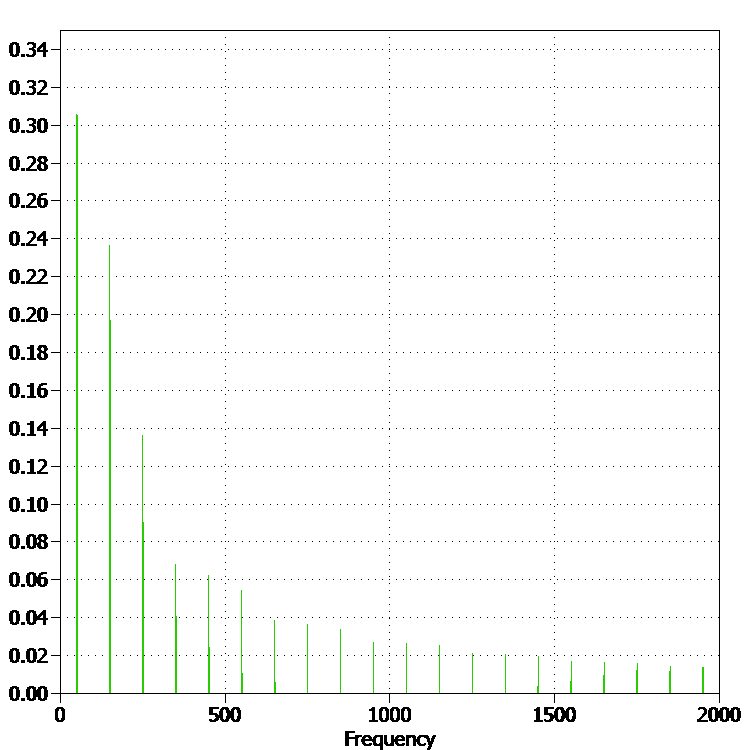
\includegraphics[width=0.32\linewidth]{plecs_phasenanschnitt_120.png}\label{fig:plecs_phasenanschnitt_120}}
	\caption{Phasenanschnitt mit 120\textdegree simuliert mit Plecs (a) Eingangssignal (b) Amplituden- und Phasenspektrum}
	\label{fig:Plecs_mit_phasenanschnitt_120}
\end{figure}


\begin{figure}[ht!]
	\centering
	\subfloat[][]{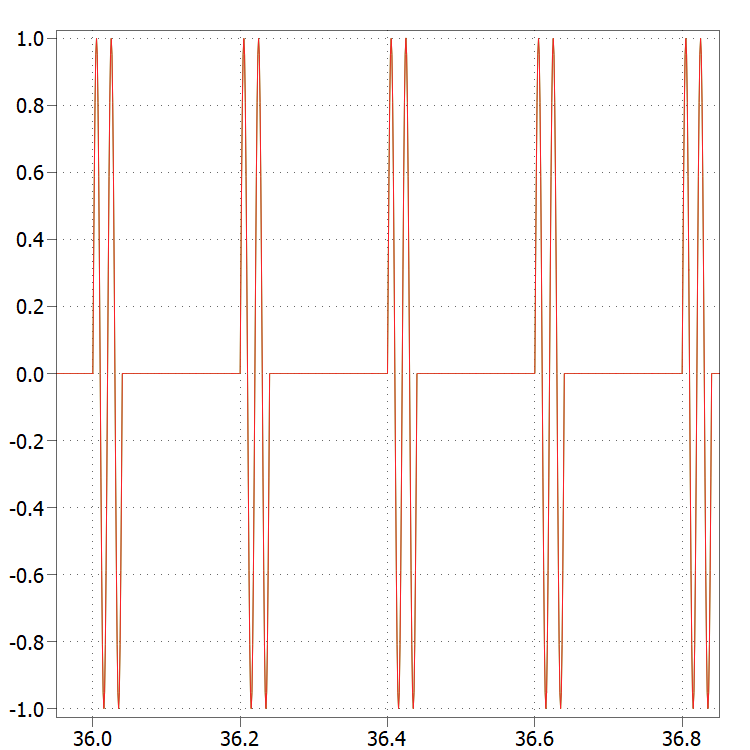
\includegraphics[width=0.32\linewidth]{plecs_schwingungspacket_0_2_schwingungen.PNG}\label{fig:plecs_schwingungspacket_0_2_schwingungen}}\qquad
	\subfloat[][]{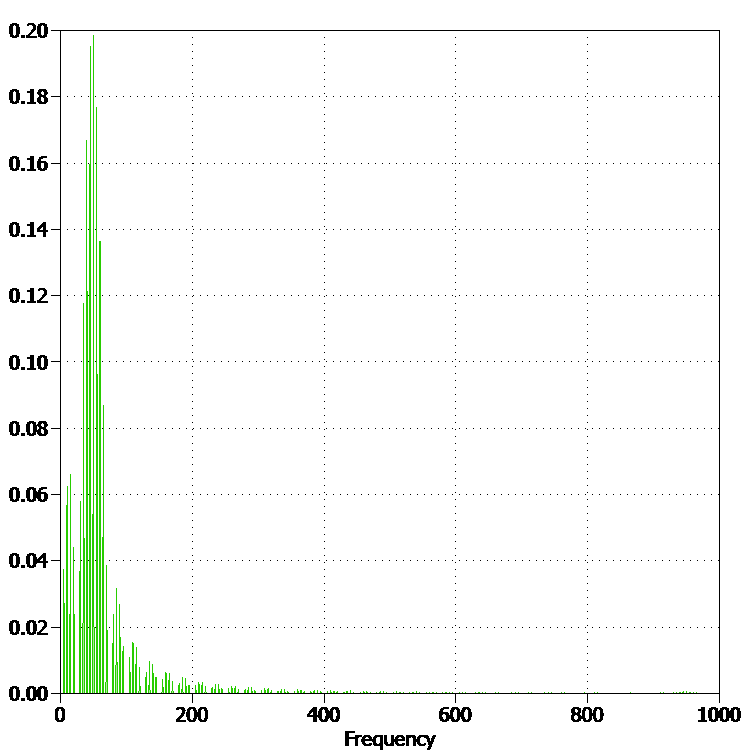
\includegraphics[width=0.32\linewidth]{plecs_schwingungspacket_0_2_1000.PNG}\label{fig:plecs_schwingungspacket_0_2_1000}}
	\caption{Schwingungspaketsteuerung mit duty cycle 0.2 simuliert mit Plecs (a) Eingangssignal (b) Amplitudenspektrum}
	\label{fig:Schwingungspaketsteuerung_mit_duty_cycle_0_2 simuliert_mit_Plecs}
\end{figure}

\newpage

\begin{figure}[ht!]
	\centering
	\subfloat[][]{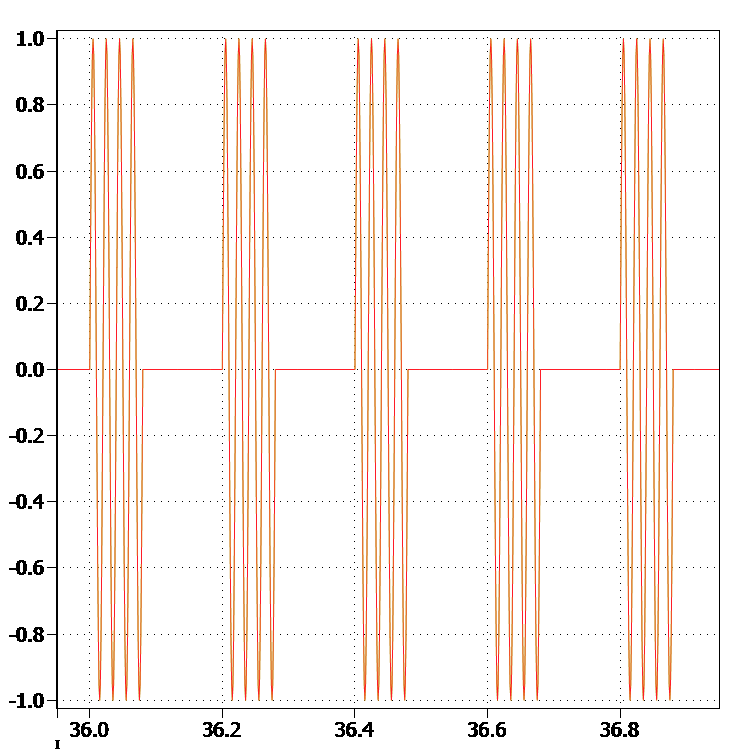
\includegraphics[width=0.32\linewidth]{plecs_schwingungspacket_0_4_schwingungen.PNG}\label{fig:plecs_schwingungspacket_0_4_schwingungen}}\qquad
	\subfloat[][]{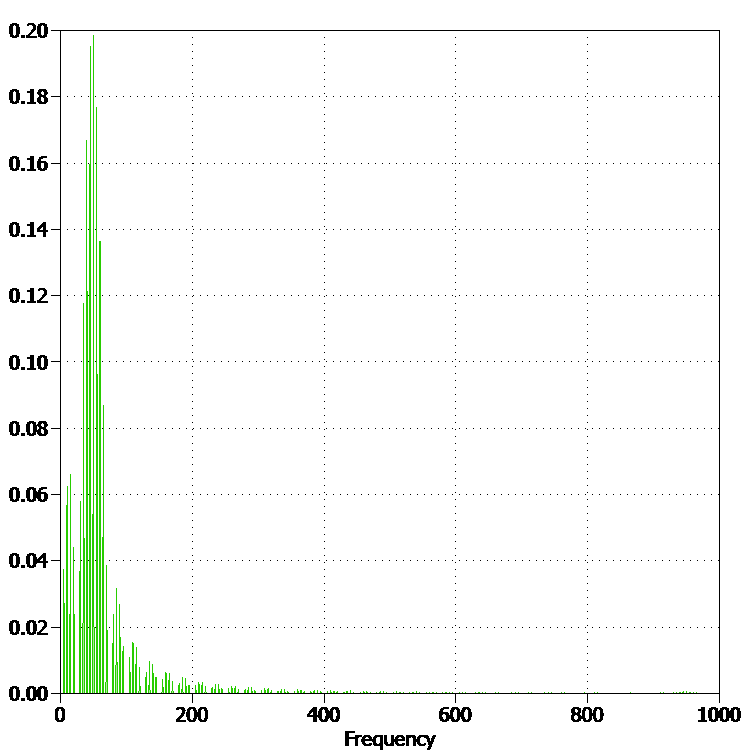
\includegraphics[width=0.32\linewidth]{plecs_schwingungspacket_0_2_1000.PNG}\label{fig:plecs_schwingungspacket_0_4_1000}}
	\caption{Schwingungspaketsteuerung mit duty cycle 0.4 simuliert mit Plecs (a) Eingangssignal (b) Amplitudenspektrum}
	\label{fig:Schwingungspaketsteuerung_mit_duty_cycle_0_4 simuliert_mit_Plecs}
\end{figure}


\begin{figure}[ht!]
	\centering
	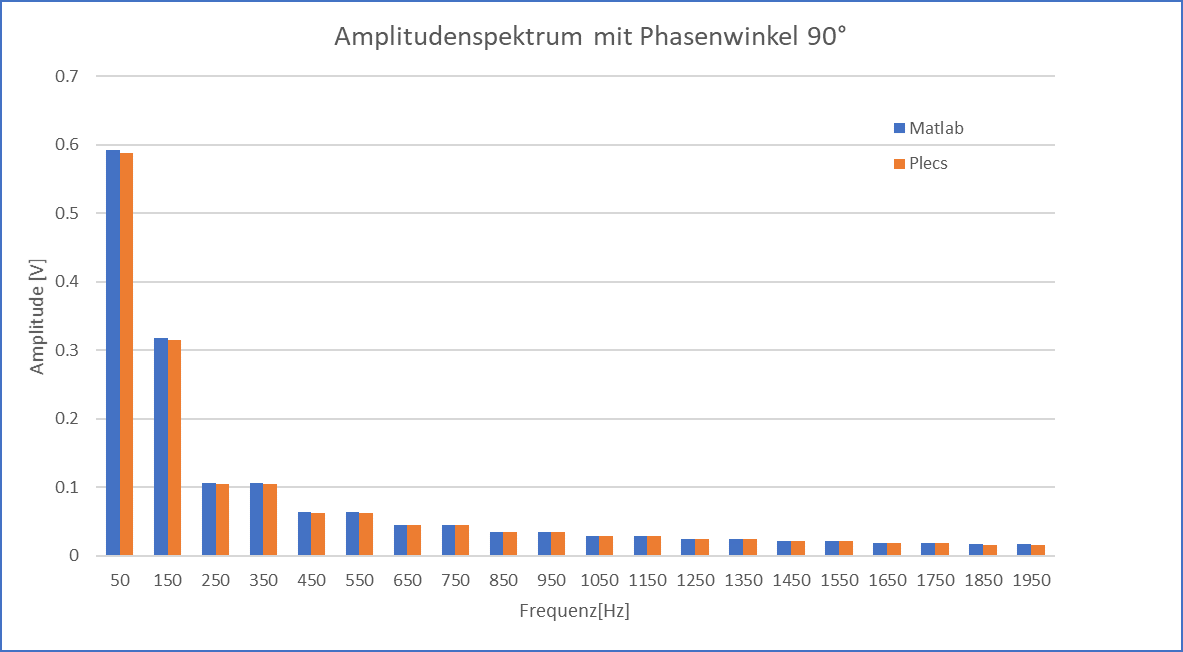
\includegraphics[scale=0.55]{Vergleich_Amplitudenspektrum_mit_Phasenwinkel_90.png}	
	\caption{Vergleich der Amplitudenspektrum mit Phasenwinkel von 90\textdegree}
	\label{fig:Vergleich_der_Amplitudenspektrum_mit Phasenwinkel_von_90}
\end{figure}

\begin{figure}[ht!]
	\centering
	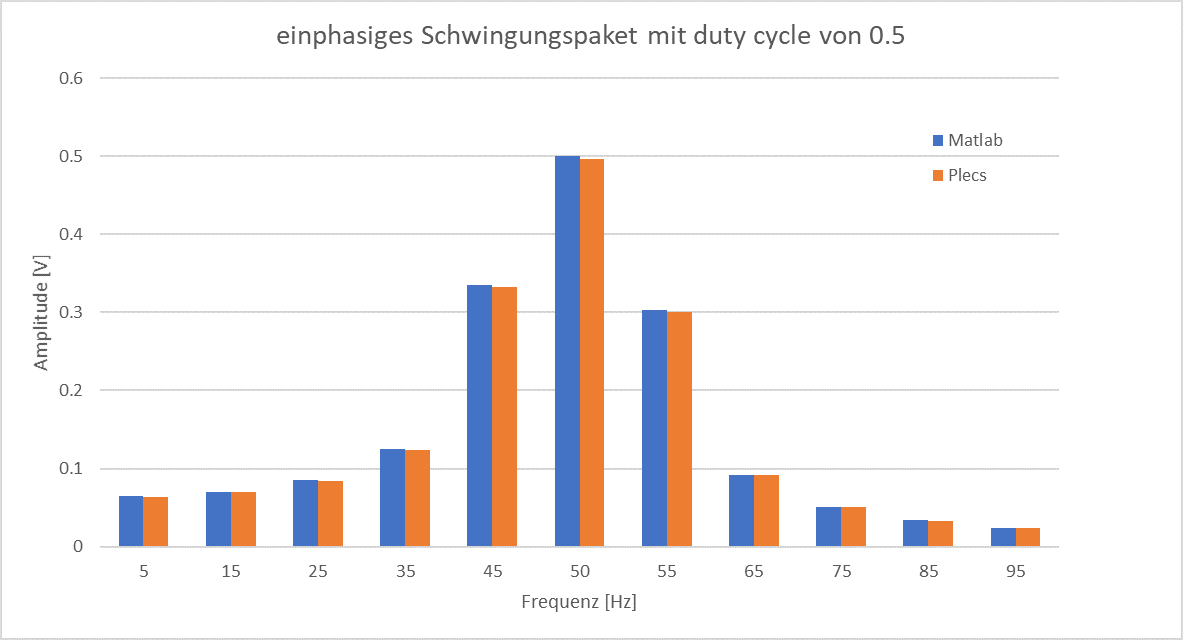
\includegraphics[scale=0.55]{Vergleich_einphasiges_Schwingungspaket_mit_duty_cycle_von_0_5.png}	
	\caption{Vergleich des Schwingungspaket mit duty cycle von 0.5}
	\label{fig:Vergleich des Schwingungspaket mit duty cycle von 0.5}
\end{figure}

\newpage

\begin{figure}[ht!]
	\centering
	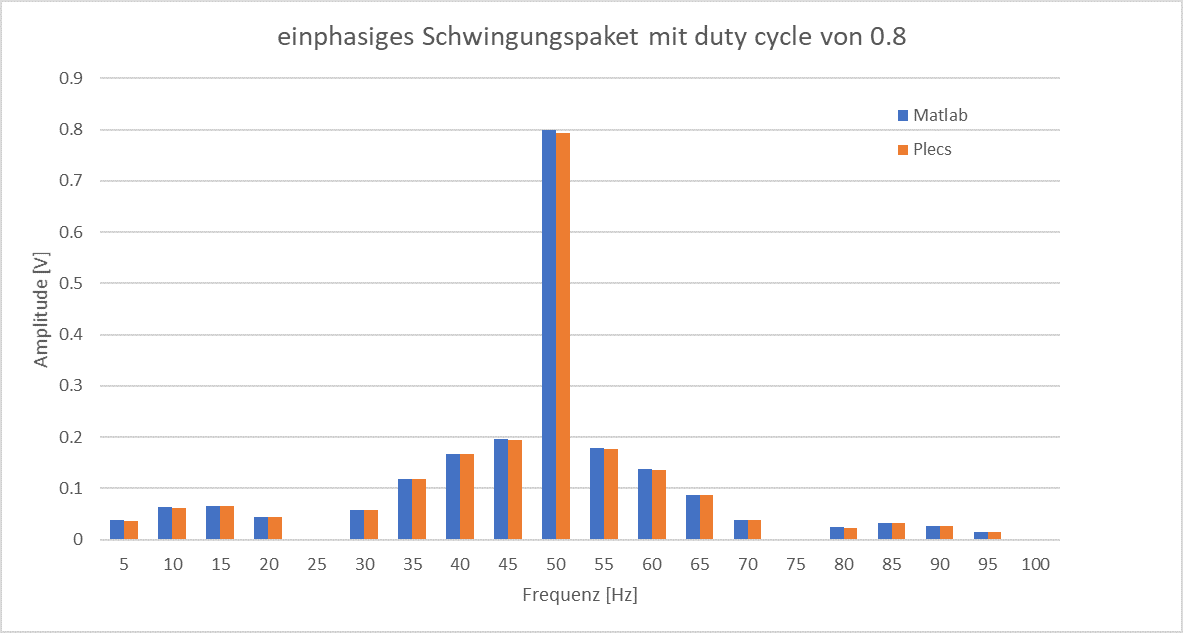
\includegraphics[scale=0.55]{Vergleich_einphasiges_Schwingungspaket_mit_duty_cycle_von_0_8.png}	
	\caption{Vergleich des Schwingungspaket mit duty cycle von 0.8}
	\label{fig:Vergleich des Schwingungspaket mit duty cycle von 0.8}
\end{figure}

\begin{figure}[ht!]
	\centering
	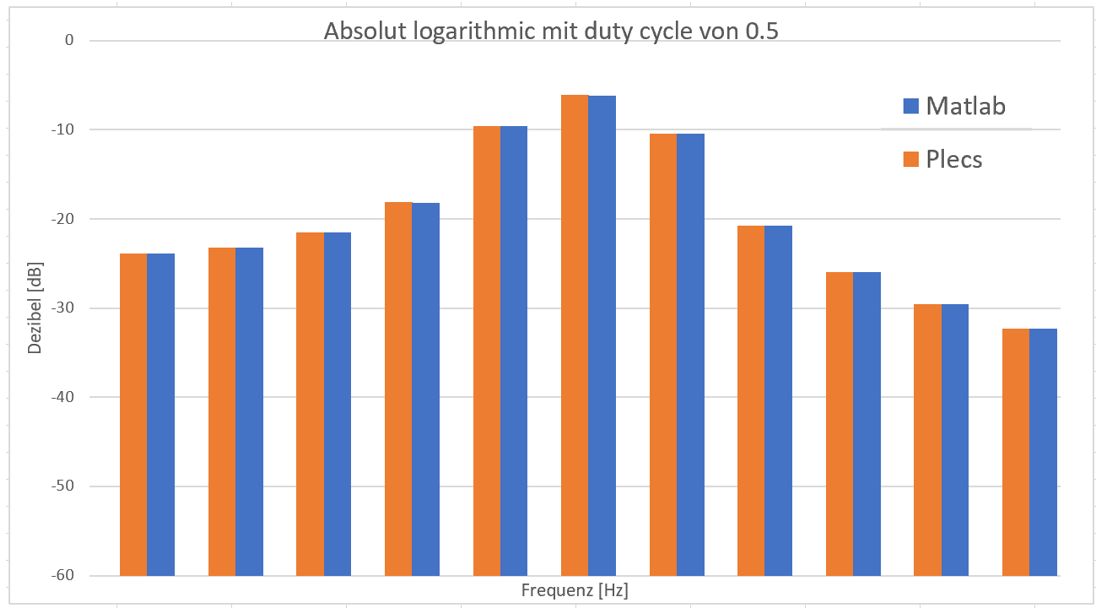
\includegraphics[scale=0.55]{Vergleich_absolut_logarithmic_duty_cycle_von_0_5_mit_legende.PNG}	
	\caption{Vergleich des Schwingungspaket mit duty cycle von 0.8}
	\label{fig:Vergleich_absolut_logarithmic_duty_cycle_von_0_5_mit_legende}
\end{figure}

\begin{figure}[ht!]
	\centering
	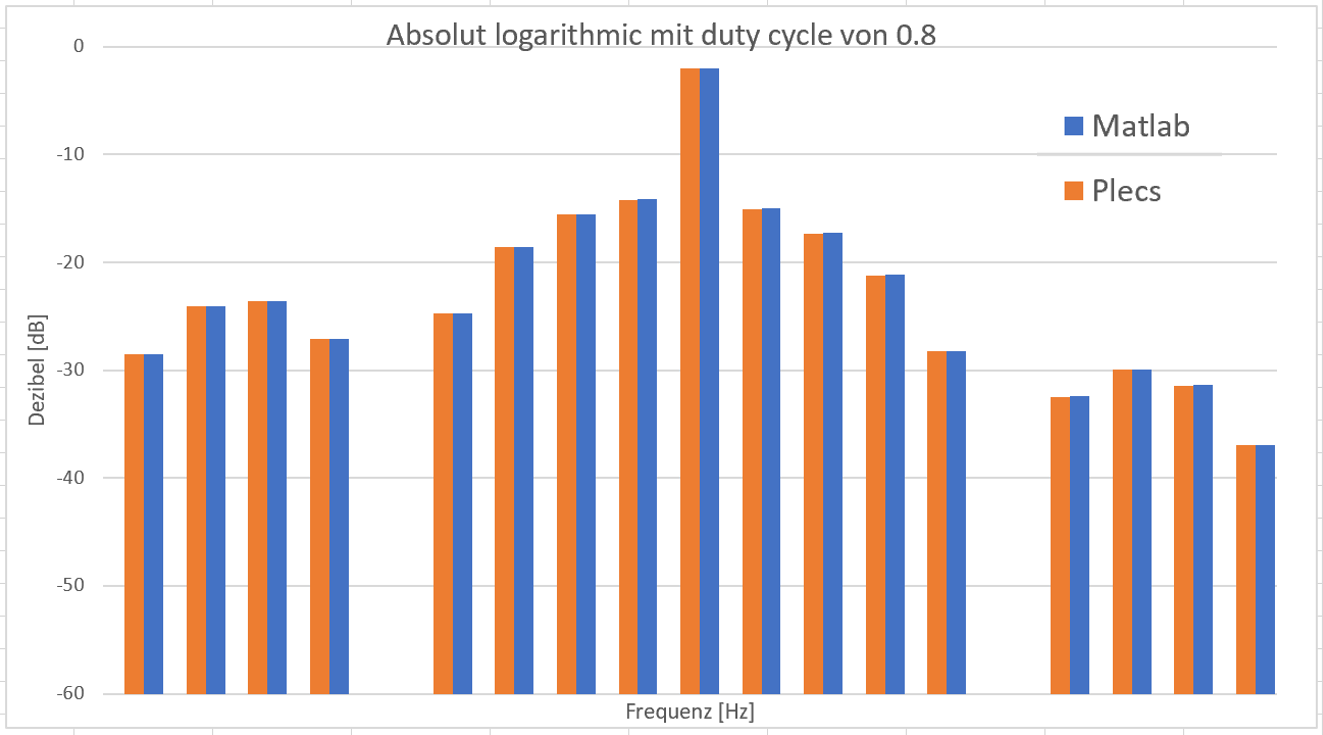
\includegraphics[scale=0.55]{Vergleich_absolut_logarithmic_duty_cycle_von_0_8_mit_legende.PNG}	
	\caption{Vergleich des Schwingungspaket mit duty cycle von 0.8}
	\label{fig:Vergleich_absolut_logarithmic_duty_cycle_von_0_8_mit_legende}
\end{figure}

\end{appendix}


